\chapter{A Gaussian mixture model}\label{ch:gmm}
In \Cref{ch:linear_theory}, we described and justified a framework for computing approximations to the solutions of nonlinear SDEs via linearisations about solutions to the corresponding deterministic system.
A key advantage of this approximation is the efficiency of computation; rather than having to generate a large number of realisations of the SDE solution we can solve a smaller system of differential equations to obtain the first two moments.
When the initial condition is fixed or Gaussian, the resulting linearisation solution is a Gaussian process, providing an approximation characterised entirely by these two moments and an analytically available probability density function.
A Gaussian approximation has further practical advantages, leading to its use across many different applications \citep{KaszasHaller_2020_UniversalUpperEstimate,ArchambeauEtAl_2007_GaussianProcessApproximations,Jazwinski_2014_StochasticProcessesFiltering,SarkkaSolin_2019_AppliedStochasticDifferential,Sanz-AlonsoStuart_2017_GaussianApproximationsSmall}.
For example, even in inference requiring Monte Carlo simulations, a Gaussian distribution with a specified mean and covariance is faster to sample from than generating numerical solutions of the nonlinear SDE.

Recall that we are interested in approximating the solution at a time \(t\) to the nonlinear stochastic differential equation
\begin{equation}
	\dif y_t = u\!\left(y_t, t\right)\dif t + \epsilon\sigma\!\left(y_t, t\right)\dif W_t,
	\label{eqn:sde_y_gmm}
\end{equation}
subject to some random initial condition \(y_s = x\), by using linearisations about solutions of the corresponding deterministic system
\begin{equation}
	\dod{F_s^t\!\left(x_0\right)}{t} = u\!\left(F_s^t\!\left(x_0\right), t\right), \quad F_s^s\!\left(x_0\right) = x_0.
	\label{eqn:det_ode_gmm}
\end{equation}
The behaviour of the solution \cref{eqn:sde_y_gmm} over the time interval \([s,t]\) for small \(\epsilon\) can be approximated by the linearised SDE
\begin{equation}
	\dif l_t = \left(u\!\left(F_s^t\!\left(x\right), t\right) + \nabla u\!\left(F_s^t\!\left(x\right), t\right)\left[l_t - F_s^t\!\left(x\right)\right]\right)\dif t + \epsilon\sigma\!\left(F_s^t\!\left(x\right), t\right)\dif W_t,
	\label{eqn:sde_linear_gmm}
\end{equation}
subject to the initial condition \(l_s = x\).
\Cref{ch:linear_theory} considered the evolution of \cref{eqn:sde_y_gmm} over a time interval \([0,t]\) and subject to some initial condition at time \(0\).
However, by using a simple time shift our theory can be applied to any finite time interval \([s,t]\), where the solution is specified at time \(s\) instead of \(0\), without loss of generality.
Note that we have now also dropped the dependence of \(\epsilon\) in the notation \(y_t\) and \(l_t\), as \(\epsilon\) is now treated as a fixed value specified as part of the model.
Suppose that the random initial condition \(x\) follows a Gaussian distribution with mean \(x_s\) and a specified covariance matrix \(\Sigma_s\).
This also permits the initial condition to be fixed as \(x_s\): we then set \(\Sigma_s = O\), the \(n \times n\) zero matrix, and follow the convention that the resulting zero-variance Gaussian is a Dirac delta centred at the mean \(x_s\).
We will focus our attention on this case for the remainder of this thesis, having already provided a general framework in \Cref{ch:linear_theory} for other initial conditions.
By taking the mean \(x_s\) as the initial condition to \cref{eqn:det_ode_gmm}, we ensure that the initial uncertainty (measured by the \(L_r\)-norm as in \Cref{ch:linear_theory}) scales with the trace of \(\Sigma_s\) (recall \cref{eqn:gauss_dist_bound}).
The solution to \cref{eqn:sde_linear_gmm} is then a Gaussian process characterised by the mean \(F_s^t\!\left(x_0\right)\) and covariance matrix \(\var{l_t}\), for which explicit expressions are given in \Cref{cor:limit_moments}.
To recall the notation used in \Cref{sec:mazzoni}, set \(w_t \equiv F_s^t\!\left(x_s\right)\) and \(\Pi_t \equiv \var{l_t}\).
When the Jacobian \(\nabla u\) of the vector field \(u\) is available or can be approximated appropriately, the moments of the Gaussian solution can be obtained by the system of ordinary differential equations
\begin{subequations}\label{eqn:gauss_de_gmm}
	\begin{align}
		\dod{w_t}{t}   & = u\!\left(w_t, t\right), \quad w_s = x_0 \label{eqn:gauss_mean_de_gmm}                                                                                                       \\
		\dod{\Pi_t}{t} & = \begin{multlined}[t]
			                   \nabla u\!\left(w_t, t\right) \Pi_t + \Pi_t\left[\nabla u\left(w_t, t\right)\right]^{\T} + \sigma\left(w_t, t \right)\sigma\left(w_t, t\right)^{\T}, \quad \Pi_s = \Sigma_s.
		                   \end{multlined}
		\label{eqn:gauss_cov_de_gmm}
	\end{align}
\end{subequations}
In practice, \cref{eqn:gauss_de_gmm} must be solved numerically, but can be more computationally efficient than the alternative of generating many realisations of \cref{eqn:sde_y_gmm}.
Thus, we can efficiently compute a Gaussian approximation \(\Gauss{w_t, \Sigma_t}\) to the solution to the nonlinear SDE \cref{eqn:sde_y_gmm} at time \(t\) by solving \cref{eqn:gauss_de_gmm} only.
The \citet{Mazzoni_2008_ComputationalAspectsContinuous} method, outlined in \Cref{sec:mazzoni}, provides a computationally efficient algorithm for solving \Cref{eqn:gauss_de_gmm} jointly.

Despite the computational appeal, this Gaussian approximation is only `reasonable' in the limit of small initial and ongoing uncertainty, which we quantified precisely with the bound in \Cref{thm:main}, and demonstrated heuristically with examples in \Cref{fig:sine_hists,fig:1d_mult_hists,fig:y_hists}.
In practice, the scale of the noise is an inherent part of a model and there is no guarantee that it is sufficiently small for this Gaussian approximation to be reasonable.
When the noise scale is larger, we see non-Gaussianity emerge---the numerical solutions in \Cref{fig:sine_hists,fig:1d_mult_hists,fig:y_hists} exhibit skewness, bi-modality, and other departures from Gaussianity.
Non-Gaussianity is also often observed in statistical measurements in practice, such as in atmospheric regimes \citep{SuraEtAl_2005_MultiplicativeNoiseNonGaussianity}, experimental fluid flows \citep{del-Castillo-Negrete_1998_AsymmetricTransportNonGaussian}, and oceanic flows \citep{BraccoEtAl_2000_VelocityProbabilityDensity}.
Although the Gaussian approximation can still provide qualitative insight into the behaviour of these solutions (see stochastic sensitivity, for instance), to produce a reasonable approximation we need a method that can capture these departures from Gaussianity.

% \section{An example: the Bene\v{s} SDE}
\begin{figure}
	\centering
	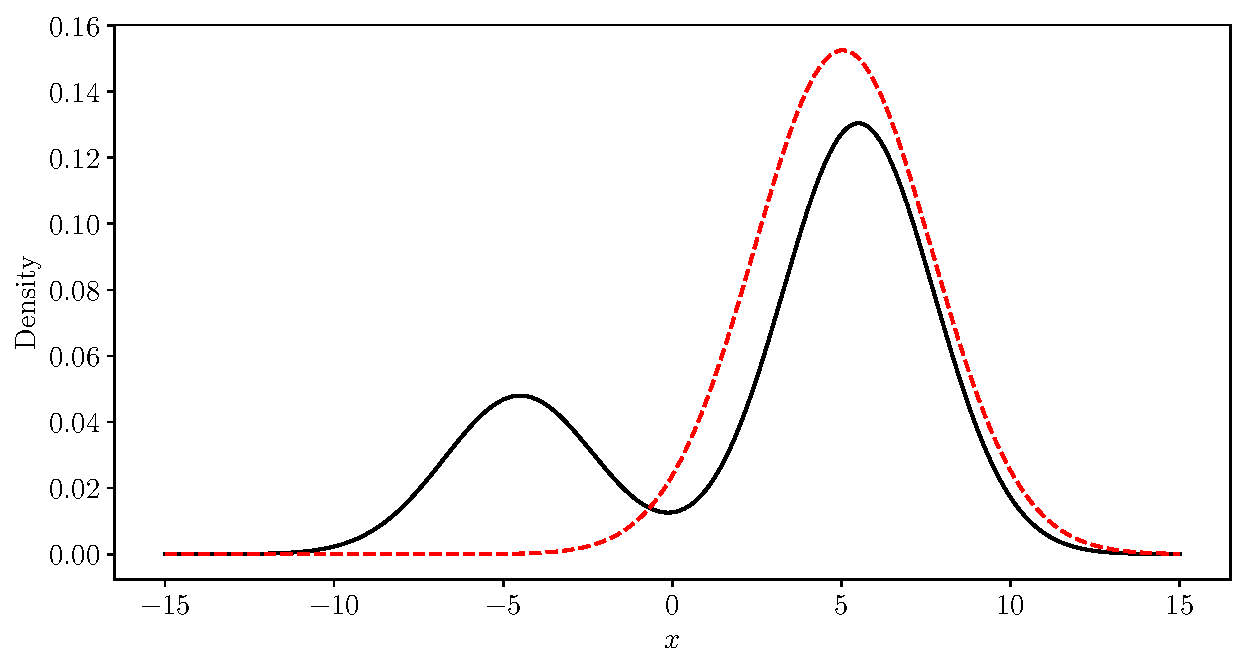
\includegraphics[width=0.9\textwidth]{chp05_gmm/figures/bene_final_gauss_5.0.pdf}
	\caption{The probability density function \cref{eqn:bene_sde_pdf} of the solution \(x_5\) (in black) to the Bene\v{s} SDE \cref{eqn:bene_sde}, with fixed initial condition \(x_0 = 1/2\).
		The density function of the Gaussian solution to the corresponding linearisation is overlaid in dashed red.}
	\label{fig:bene_gauss}
\end{figure}

To further illustrate this point, we consider another example of a 1-dimensional stochastic differential equation.
The Bene\v{s} SDE \citep{SarkkaSolin_2019_AppliedStochasticDifferential} is
\begin{equation}
	\dif x_t = \tanh\!\left(x_t\right)\dif t + \dif W_t.
	\label{eqn:bene_sde}
\end{equation}
We are implicitly taking \(\epsilon = 1\), which is a larger noise scale than we typically expect to apply our results to.
However, this example is purely demonstrative to highlight a limitation of Gaussian approximations and show the potential of the algorithm we are about to propose; later examples will involve smaller values of \(\epsilon\).
The deterministic system corresponding to \cref{eqn:bene_sde} is
\begin{equation}
	\dod{F_s^t\!\left(x\right)}{t} = \tanh\!\left(F_s^t\!\left(x\right)\right), \quad F_s^s\!\left(x\right) = x,
	\label{eqn:bene_ode}
\end{equation}
which includes an unstable fixed point at \(0\).
The solution to \cref{eqn:bene_ode} over the time interval \((s,t)\) is
\begin{equation}
	F_s^t\!\left(x\right) = \arcsinh\!\left(e^{t-s}\sinh\!\left(x\right)\right).
	\label{eqn:bene_ode_sol}
\end{equation}
The probability density function of the weak solution to \cref{eqn:bene_sde} can be derived using an appropriate change of measure with Girsanov's theorem (see Section 7.3 of \citet{SarkkaSolin_2019_AppliedStochasticDifferential}).
The solution \(x_t\) at time \(t\) has the probability density function
\begin{equation}\label{eqn:bene_sde_pdf}
	p(x,t) = \frac{1}{\sqrt{2\pi t}}\frac{\cosh\!\left(x\right)}{\cosh\!\left(x_0\right)}\exp\left[-\frac{t}{2} - \frac{1}{2t}\left(x - x_0\right)^2\right],
\end{equation}
where \(x_0\) is the fixed initial condition.
In this example, we consider the solution to \cref{eqn:bene_sde} subject to the fixed initial condition \(x_0 = 1/2\) and at time \(t = 5\) and plot the resulting PDF of the solution \cref{eqn:bene_sde_pdf} in black in \Cref{fig:bene_gauss}.
The density is not symmetric with two distinct modes that result from the unstable fixed point of \cref{eqn:bene_ode} at \(x = 0\).
Many stochastic trajectories are driven away from zero, resulting in the predominant mode centred at \(x = 11/2\).
However, when the stochastic perturbations force a trajectory through the fixed point and into negative values, they are pushed further in the negative direction, leading to the second mode at \(x = -9/2\).
Nonetheless, we can linearise \cref{eqn:bene_sde} about the deterministic trajectory \(F_0^t\!\left(1/2\right)\) solving \cref{eqn:bene_ode} to obtain a Gaussian approximation.
In general, if we linearise \cref{eqn:bene_sde} over the time interval \([s,t]\) about the trajectory \(F_s^t\!\left(x_s\right)\), we are considering the equation
\[
	\dif l_t = \left(\tanh\!\left(F_s^t\!\left(x_s\right)\right) + \arcsech\!\left(F_0^t\!\left(x_s\right)\right)\left[l_t - F_s^t\!\left(x_s\right)\right]\right)\dif t + \dif W_t,
\]
where the deterministic flow map \(F_s^t\) given by \cref{eqn:bene_ode_sol}.
Since the deterministic flow map is available analytically in \cref{eqn:bene_ode_sol}, we can determine the variance of the solution to the linearised SDE exactly by evaluating \cref{eqn:pi_expl_eqn}.
% This computation gives
% \[
% 	\var{l_t} = \frac{2\sinh^2\!\left(x_s\right)\left(t - s\right) + e^{2t - 2s} - 1}{2\sinh^2\!\left(x_0\right) + 2e^{2s - 2t}},
% \]
% with details provided in \Cref{app:bene_calculations}.
The solution to \cref{eqn:bene_sde} at time \(t\) is then approximated by the Gaussian distribution
\[
	l_t \sim \mathcal{N}\!\left(\arcsinh\!\left(e^{t - s} \sinh\!\left(x_s\right)\right),\, \frac{2\sinh^2\!\left(x_s\right)t + e^{2t - 2s} - 1}{2\sinh^2\!\left(x_s\right) + 2e^{-2s-2t}}\right).
\]
Returning to our specific example (\(x_0 = 1/2\), \(s = 0\), and \(t = 5\)), we plot the density of the Gaussian approximation \(l_5\) in dashed red in \Cref{fig:bene_gauss}.
The Gaussian approximation cannot capture the bimodality of the true solution, and so only a single mode is captured.
This is a significant limitation of using a single linearisation approximation.


To improve upon the single linearisation approximation, we  seek a scheme that can capture departures from Gaussianity in the SDE solution, while still taking advantage of the efficient computation of the linearisation solution.
An alternative perspective is that the linearised SDE captures the behaviour of stochastic fluctuations close to a deterministic trajectory, in a similar sense to how a Taylor polynomial captures the local behaviour of a nonlinear function.
By `piecing' together several of these approximations together we can capture the stochastic behaviour in different regions of the state space.
A Gaussian mixture model (GMM) provides a framework for combining multiple Gaussian densities into a single distribution and is thus the obvious choice for constructing non-Gaussian densities out of our Gaussian approximations.
In this chapter, we outline an algorithm that uses \emph{multiple} linearisation approximations to construct a Gaussian mixture model that approximates the nonlinear SDE solution.
% The algorithm itself is provided in \Cref{sec:gmm_alg}.

% Helper functions for TikZ pic
\newcommand{\TikZGauss}[3]{1 / sqrt(2 * pi * #3) * exp(-(#1 - #2) * (#1 - #2) / #3)} % Args: variable, mean, variance
\newcommand{\TikZMixtureTwo}[8]{% Args: width, comp1_mean, comp1_var, comp2_mean, comp2_var, comp1_weight, comp2_weight, vertical scaling
	\begin{tikzpicture}
		% Two components
		\draw[domain=0:#1, smooth, variable=\x, dashed] plot ({\x}, {#8 * \TikZGauss{\x}{#2}{#3}});
		\draw[domain=0:#1, smooth, variable=\x, dashed] plot ({\x}, {#8 * \TikZGauss{\x}{#4}{#5}});
		% Mixture model
		\draw[domain=0:#1, smooth, variable=\x, very thick] plot ({\x}, {#8 * #6 * \TikZGauss{\x}{#2}{#3} + #8 * #7 * \TikZGauss{\x}{#4}{#5}});
		\draw[thick] (0,0)--(#1,0);
	\end{tikzpicture}
}

\begin{figure}
	\centering
	\begin{subfigure}{0.49\textwidth}
		\TikZMixtureTwo{7}{2}{1}{3}{2}{0.5}{0.5}{3}
		\caption{Skewness}
	\end{subfigure}
	\begin{subfigure}{0.49\textwidth}
		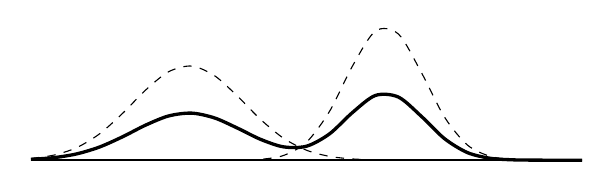
\begin{tikzpicture}
			\TikZMixtureTwo{7}{2}{1}{4.5}{0.5}{0.5}{0.5}{3}
		\end{tikzpicture}
		\caption{Bimodality}
	\end{subfigure}
	\caption{The probability density functions of two Gaussian mixture models in 1-dimension both using two equally weighted components.
		When individual components (dashed) are combined to produce non-Gaussian mixture densities (solid), they can exhibit both (a) skewness and (b) bimodality.}
	\label{fig:mixture_model}
\end{figure}

In general, a Gaussian mixture model with \(K\) components is a probability density function of the form
\[
	p(z) = \sum_{k=1}^{K}{\omega_k \Gauss{z;\, \mu^{(k)}, \Sigma^{(k)}}},
\]
consisting of \(K\) Gaussian components \(\Gauss{\mu^{(k)}, \Sigma^{(k)}}\) with respective weights \(\omega_1, \dotsc, \omega_K \geq 0\) that satisfy \(\sum_{k=1}^{K}\omega_k = 1\).
With sufficient components, a Gaussian mixture model can recreate any probability distribution in \(\R^n\) while having many of the properties that make Gaussian distributions appealing in practice \citep{McLachlanEtAl_2019_FiniteMixtureModels}.
\Cref{fig:mixture_model} shows two examples of Gaussian mixture models in 1-dimension, where departures from Gaussianity such as multimodality and skewness can be captured with an appropriate combination of components.



\section{The GMM algorithm}\label{sec:gmm_alg}
We will now outline our algorithm to approximate the SDE solution with a Gaussian mixture model while taking advantage of the computational efficiency of the Gaussian linearisation approximation.
Given a Gaussian component at a time \(s\), we can `propagate' the component forward to a later time \(t\) by solving \Cref{eqn:gauss_de_gmm} initialised with the component mean and covariance matrix.
% That is, we are updating the mean and covariance of the Gaussian component by approximating the solution to the original SDE \cref{eqn:sde_y_gmm} over \((s,t)\) with a linearisation about the deterministic trajectory initialised from the component mean.
Given a mixture model with multiple Gaussian components, we can propagate each component \emph{separately} to update the full model through time in a computationally efficient manner.
Each component is propagated by approximating the original SDE \cref{eqn:sde_y_gmm} with a different linearisation, about the deterministic trajectory resulting from the component mean.

Our proposed method is \emph{ad hoc} and based on an intuition: the Gaussian solution provides a reasonable approximation for the local behaviour of the true SDE solution over a short timeframe, but once this is no longer the case, we can capture departures from Gaussianity by introducing more components in the mixture model.
We expect heuristically that as the number of components increases, the full mixture model should provide a closer approximation of the SDE solution density, provided that the components are appropriately placed.
However, our goal is to provide a numerically efficient algorithm, so we wish to minimise the number of components and use the Gaussian approximation wherever possible.
We therefore propose propagating Gaussian components forward through the linearisation model until are no longer reasonable approximations of the local solution behaviour.
Then, we replace the violating component with several smaller judiciously chosen components and propagate each new component individually.
We term this the \emph{splitting} step, where a Gaussian component is split into several smaller ones.
The new components should be chosen in such a way as to `preserve' the original component, which can be achieved in one sense as follows.
Let \(\Xi\) follow a Gaussian mixture density with \(N\) components, with respective weights \(w^{(1)}, \dotsc, w^{(N)}\), means \(\mu^{(1)},\dotsc,\mu^{(N)}\), and covariance matrices \(\Sigma^{(1)},\dotsc,\Sigma^{(N)}\).
The variance of the mixture model is then
\begin{align*}
	\var{\Xi} & = \sum_{i=1}^{N}{w^{(i)}\Sigma^{(i)}} + \sum_{i=1}^{N}{w^{(i)}\left(\mu^{(i)} - \bar{\mu}\right)\left(\mu^{(i)} - \bar{\mu}\right)^{\T}} \\
	          & = \text{Mean of covariances} + \text{Covariance of means},
\end{align*}
where \(\bar{\mu} = \avg{\Xi} = \sum_{i=1}^{N}{w^{(i)}\mu^{(i)}}\) is the overall mean.
This decomposition suggests, at least heuristically, that we can include additional uncertainty (in the form of contributions to the overall variance) within the component means themselves.
By replacing a single component with points, we can preserve the mean and covariance of the component while introducing additional components that can closely match the non-Gaussian target distribution.
This leads to the following condition: the \(K\) splitting points (the new component means) \(x^{(1)}, \dotsc, x^{(K)}\) that replace \(x\) should be chosen so that
\begin{equation}
	\sum_{i=1}^K{\hat{w}_k x^{(k)}} = x, \quad \sum_{i=1}^{K}{\hat{w}_k\left(x^{(k)} - x\right)\!\left(x^{(k)} - x\right)^{\T}} = \Sigma_0.
	\label{eqn:cov_split_points}
\end{equation}
with weights \(\hat{w}_1,\dotsc,\hat{w}_K > 0\) satisfying \(\sum_{k=1}^{K}{\hat{w}_k} = 1\).
Each new component is assigned a zero variance in this formulation, but with an appropriate adjustment of \cref{eqn:cov_split_points} each can have a specified variance.
This ensures that the mean and covariance of the original Gaussian are preserved within the (sample) mean and covariance of the new points themselves.
Note that at least \(K = n + 1\) points are necessary for \cref{eqn:cov_split_points} to be satisfied.
The selection of splitting points is similar to the notion of `sigma points', employed in the unscented transform to encode an initial mean and covariance \citep{Uhlmann_1995_DynamicMapBuilding,JulierEtAl_2000_NewMethodNonlinear}.
Any such sigma points satisfy \cref{eqn:cov_split_points}---Table I in \citet{MenegazEtAl_2015_SystematizationUnscentedKalman} provides a list of sigma points and their weightings used across other literature (and reviewed in the context of Kalman filtering)---and therefore can be used in our algorithm.
% However, we note a key difference between our proposed algorithm and the unscented transform; the unscented transform provides an \emph{exact} estimate of.

\begin{figure}
	\centering
	\begin{tikzpicture}[rotate=25, scale=1.5]
		% Ellipse
		\draw[black] (0,0) ellipse (70pt and 40pt);
		\node[black, anchor=west, xshift=2pt] at ($(0,0)+(-40:70pt and 40pt)$) {\(\Sigma_0\)};

		% Reference lines
		\draw[dashed, gray] ($(0,0)+(90:70pt and 40pt)$) -- (0,0)
		($(0,0)+(0:70pt and 40pt)$) -- (0,0)
		($(0,0)+(-90:70pt and 40pt)$) -- (0,0)
		($(0,0)+(180:70pt and 40pt)$) -- (0,0);

		% Points
		\fill[black] (0,0) circle[radius=1pt] node[anchor = west] {\(x = {\color{blue}{x^{(1)}}}\)};
		\fill[blue] ($(0,0)+(90:70pt and 40pt)$) circle[radius=1pt] node[anchor=south] {\(x^{(2)}\)};
		\fill[blue] ($(0,0)+(0:70pt and 40pt)$) circle[radius=1pt] node[anchor=west] {\(x^{(3)}\)};
		\fill[blue] ($(0,0)+(-90:70pt and 40pt)$) circle[radius=1pt] node[anchor=north] {\(x^{(4)}\)};
		\fill[blue] ($(0,0)+(180:70pt and 40pt)$) circle[radius=1pt] node[anchor=east] {\(x^{(5)}\)};
	\end{tikzpicture}
	\caption{The splitting of a 2-dimensional mean \(x\) and \(2\times 2\) covariance matrix \(\Sigma\) (in black) into 5 sigma points \(x^{(1)}, \dotsc, x^{(5)}\) (in blue), using the canonical set \cref{eqn:uhlman_sigma}.
		The mean \(x\) is preserved as one of the points, and the four others are placed at the vertices and co-vertices of the first standard deviation ellipse of \(\Sigma\).}
	\label{fig:sigma_points_ex}
\end{figure}

The canonical set of sigma points originally proposed by \citet{Uhlmann_1995_DynamicMapBuilding}, which we use to apply the GMM algorithm in \Cref{ch:appls}, are
\begin{subequations}\label{eqn:uhlman_sigma}
	\begin{align}
		x^{(1)}         & = x,                                                          \\
		x^{(1 + i)}     & = x + \sqrt{n + \frac12}\left[\sqrt{\Sigma}\right]_{\cdot i}, \\
		x^{(1 + n + i)} & = x - \sqrt{n + \frac12}\left[\sqrt{\Sigma}\right]_{\cdot i},
	\end{align}
\end{subequations}
for \(i = 1,\dotsc, n\), where \(\sqrt{\Sigma}\) denotes the symmetric square root of \(\Sigma\), and \(\left[\sqrt{\Sigma}\right]_{\cdot i}\) denotes the \(i\)th column of \(\sqrt{\Sigma}\).
The points are uniformly weighted, i.e.\ \(\hat{w}_k = 1 / (2n + 1)\).
\Cref{fig:sigma_points_ex} depicts the splitting of a mean and covariance matrix pair into 5 sigma points in 2-dimensions, using the canonical set \cref{eqn:uhlman_sigma}.
By perturbing the mean by the columns of the square root of the covariance matrix, the sigma points are placed at the vertices of the ellipse representing the matrix.
However, we do not enforce a particular approach for selecting these points and leave this to be investigated further as future work.

The two critical steps of the algorithm are \emph{when} to split, a criterion that should decide when the Gaussian approximation is no longer a reasonable representation of the nearby solution behaviour, and \emph{how} to split, with the appropriate method that ensures the new components satisfy \cref{eqn:cov_split_points}.
We do not provide specific choices for either step and save a thorough investigation for future work.
In \Cref{sec:gmm_split_disc}, we do however include a brief discussion of some options for the splitting criterion.

The mixture model algorithm is as follows:
\begin{enumerate}
	\item Initialise a Gaussian mixture model with \(N\) components, setting \(x^{(1)},\dotsc, x^{(N)}\) to be the component means, \(\Sigma^{(1)}, \dotsc, \Sigma^{(N)}\) to be the component covariance matrices, and \(w^{(1)}, \dotsc, w^{(N)}\) to be the component weights.
	      For a fixed initial condition \(x_0\), set \(N = 1\), \(x^{(1)} = x_0\), \(\Sigma^{(1)} = O\) and \(\omega^{(1)}\).
	      Otherwise, the components and weights are represent the random initial distribution.
	      Set \(\tau^{(1)} = \dotsb = \tau^{(N)}\).

	\item While \(\tau^{(i)} < t\) for any \(i = 1,\dotsc, N\), iterate the following;

	      \begin{enumerate}
		      \item Set \(j\) to be any \(i\) for which \(\tau^{(i)} < T\).

		      \item Update \(x^{(j)}\) and \(\Sigma^{(j)}\) by solving the joint system \cref{eqn:gauss_de_gmm} with initial state \(x^{(j)}\) and covariance \(\Sigma^{(j)}\), terminating when a split condition is met or the final time \(T\) is reached.
		            Set \(\tau^{(j)}\) to the time at which this solution terminates.

		      \item If \(\tau^{(j)} = t\), then complete this branch of the algorithm.

		      \item Otherwise, if \(\tau^{(j)} < t\), construct \(K\) points \(\hat{x}^{(1)},\dotsc,\hat{x}^{(K)}\) with corresponding weights \(\hat{w}^{(1)}, \dotsc, \hat{w}^{(K)}\) that preserve the propagated mean and covariance (i.e.\ satisfying \cref{eqn:cov_split_points}).
		            Set \(x^{(j)} = \hat{x}^{(1)}\) and \(\Sigma^{(j)} = O\), and for each \(k = 2,\dotsc,K\):
		            \begin{align*}
			            \Sigma^{(N + k - 1)} & = O                     \\
			            w^{(N + k - 1)}      & = \hat{w}^{(k)} w^{(j)} \\
			            \tau^{(N + k - 1)}   & = \tau^{(j)}.
		            \end{align*}
		            Update the weight of the first sigma point as \(w^{(j)} = \hat{w}^{(1)} w^{(j)}\), and set \(N = N + K - 1\).
	      \end{enumerate}

	\item Construct the final mixture model with density function
	      \[
		      G\!\left(x\right) = \sum_{i=1}^{N}{w^{(i)}\Gauss{x; \, x^{(i)}, \Sigma^{(i)}}}.
	      \]

\end{enumerate}

\begin{figure}
	\centering
	\begin{subfigure}{\textwidth}
		\begin{tikzpicture}
			\draw (1,1.5) .. controls (3,3.5) and (5,-1.5) .. (7,1.5);

			% Initial position
			\fill[black] (1,1.5) circle[radius=1pt] node[anchor = east] {\(x\)};

			% Initial covariance
			\draw[dashed, rotate around = {58: (1, 1.5)}, blue] (1,1.5) ellipse (14pt and 22pt);
			\node[blue] at ($(1,1.5)+(90:14pt and 22pt)$) {\(\Sigma\)};

			% Mapped position
			\fill[black] (7,1.5) circle[radius=1pt] node[anchor = south] {\(w_t\)};
			\node[blue] at ($(1,1.5)+(90:14pt and 22pt)$) {\(\Sigma\)};

			% Covariance ellipse
			\draw[dashed, rotate around = {30: (7,1.5)}, red] (7,1.5) ellipse (30pt and 70pt);
			\node[red] at ($(7,1.5)+(75:30pt and 70pt)$) {\(\Pi_t\)};
		\end{tikzpicture}

		\caption{The mean \(x\) and covariance matrix \(\Sigma\) of the component is propagated forward by solving \cref{eqn:gauss_de_gmm} to obtained \(w_t\) and \(\Pi_t\) respectively.}
	\end{subfigure}
	\begin{subfigure}{\textwidth}
		\begin{tikzpicture}
			% Trajectory
			\draw[gray] (1,-4) .. controls (3,-2) and (5,-7) .. (7,-4);

			% Initial position
			\fill[gray] (1,-4) circle[radius=1pt] node[anchor = east] {\(x\)};

			% Mapped position
			\fill[blue] (7,-4) circle[radius=1pt];

			% Covariance ellipse
			\draw[dashed, rotate around = {30: (7,-4)}, gray] (7,-4) ellipse (30pt and 70pt);

			% Additional sigma points
			\fill[blue, rotate around = {30: (7,-4)}] ($(7, -4)+(0:30pt and 70pt)$) circle[radius=1pt];
			\fill[blue, rotate around = {30: (7,-4)}] ($(7, -4)+(90:30pt and 70pt)$) circle[radius=1pt];
			\fill[blue, rotate around = {30: (7,-4)}] ($(7, -4)+(180:30pt and 70pt)$) circle[radius=1pt];
			\fill[blue, rotate around = {30: (7,-4)}] ($(7, -4)+(270:30pt and 70pt)$) circle[radius=1pt];

			\draw[dashed, gray, rotate around = {30: (7,-4)}] ($(7,-4)+(0:30pt and 70pt)$) -- (7,-4)
			($(7, -4)+(90:30pt and 70pt)$) -- (7,-4)
			($(7, -4)+(180:30pt and 70pt)$) -- (7,-4)
			($(7, -4)+(270:30pt and 70pt)$) -- (7,-4);
		\end{tikzpicture}

		\caption{Once the splitting criterion is met, the mapped component is split into \(K\) new components with corresponding means (in blue) satisfying \cref{eqn:cov_split_points}.}
	\end{subfigure}
	\begin{subfigure}{\textwidth}
		\begin{tikzpicture}
			\fill[blue] (3,-13) circle[radius=1pt];
			\fill[blue, rotate around = {30: (3,-13)}] ($(3,-13)+(0:30pt and 70pt)$) circle[radius=1pt];
			\fill[blue, rotate around = {30: (3,-13)}] ($(3,-13)+(90:30pt and 70pt)$) circle[radius=1pt];
			\fill[blue, rotate around = {30: (3,-13)}] ($(3,-13)+(180:30pt and 70pt)$) circle[radius=1pt];
			\fill[blue, rotate around = {30: (3,-13)}] ($(3,-13)+(270:30pt and 70pt)$) circle[radius=1pt];

			% New trajectories
			\draw[black,  rotate around = {30: (3,-13)}] ($(3,-13)+(90:30pt and 70pt)$) .. controls (5,-14) and (8, -12) .. (10, -13);
			\draw[black,  rotate around = {30: (3,-13)}] ($(3,-13)+(0:30pt and 70pt)$) .. controls (5,-15) and (8, -12) .. (10, -14.5);
			\draw[black] (3,-13) .. controls (5,-15) and (8, -10) .. (12, -11.75);
			\draw[black,  rotate around = {30: (3,-13)}] ($(3,-13)+(180:30pt and 70pt)$) .. controls (5,-17) and (7, -15) .. (10, -18);
			\draw[black,  rotate around = {30: (3,-13)}] ($(3,-13)+(270:30pt and 70pt)$) .. controls (5,-17) and (7, -15) .. (8, -18);

			% Mapped points
			\fill[black, rotate around = {30: (3,-13)}] ($(10,-13)$) circle[radius=1pt];
			\fill[black, rotate around = {30: (3,-13)}] ($(10,-14.5)$) circle[radius=1pt];
			\fill[black] (12,-11.75) circle[radius=1pt];
			\fill[black, rotate around = {30: (3,-13)}] ($(10,-18)$) circle[radius=1pt];
			\fill[black, rotate around = {30: (3,-13)}] ($(8,-18)$) circle[radius=1pt];

			% Updated ellipses
			\draw[dashed, rotate around = {30: (3, -13)}, red] (10,-13) ellipse[x radius=30pt, y radius=70pt, rotate=75];
			\draw[dashed, rotate around = {30: (3, -13)}, red] (10,-14.5) ellipse[x radius=20pt, y radius=70pt, rotate=68];
			\draw[dashed, red] (12,-11.75) ellipse[x radius=10pt, y radius=50pt, rotate=70];
			\draw[dashed, rotate around = {30: (3, -13)}, red] (10,-18) ellipse[x radius=21pt, y radius=70pt];
			\draw[dashed, rotate around = {30: (3, -13)}, red] (8,-18) ellipse[x radius=10pt, y radius=50pt, rotate=15];

		\end{tikzpicture}

		\caption{Each new component is propagated forward with \cref{eqn:gauss_de_gmm} and the process is repeated for each component \emph{individually} until the final time is reached.}
	\end{subfigure}

	\caption{The propagation and splitting of a component in the Gaussian mixture model}
	\label{fig:gmm_steps}
\end{figure}

\begin{figure}
	\centering
	\begin{tikzpicture}[node distance=70pt]
		\tikzstyle{arrow} = [->,>=stealth]

		\node (s) [rectangle, rounded corners, draw=black, align=center] {\textbf{Start} \\ Given \(x_0, t\) };

		\node (a) [rectangle, below of=s, draw=black, align=center, yshift=-10pt] {\textbf{Initialise} \\ Set \(K = 1\) \\ Set \(x^{(1)} = x_0\) \\ Set \(\Sigma^{(1)} = O\) \\ Set \(w^{(1)} = 1\) \\ Set \(\tau^{(1)} = 0\)};

		\node (b) [diamond, below of=a, draw=black, align=center, yshift=-70pt] {Any \(i\) for \\ which \(\tau^{(i)} < t\)?};

		\node (c) [rectangle, below of=b, draw=black, align=center, yshift=-70pt] {\textbf{Propagate} \\ Update \(x^{(i)}, \Sigma^{(i)}\) by solving \\ \cref{eqn:gauss_de_gmm} from time \(\tau^{(i)}\) until \\ time \(t\) \textbf{or} the splitting \\ criterion is reached. \\
			Set \(\tau^{(i)}\) to the propagated time};

		\node (d) [diamond, right of=c, draw=black, align=center, xshift = 90pt] {\(\tau^{(i)} = t\)?};

		\node (e) [rectangle, below of = c, draw=black, align=center, yshift = -80pt] {\textbf{Split} \\ Use the splitting method (i.e.\ \cref{eqn:cov_split_points}) \\
			to set \(x^{(i)}\) and \(x^{(N + 1)}, \dotsc, x^{(N + K - 1)}\) \\
			and the corresponding weights \(w^{(i)}\) \\
			and \(w^{(N+1)}, \dotsc w^{(N + K - 1)}\). \\
			Set \(\Sigma^{(N + 1)} = \dotsb = \Sigma^{(N + K - 1)} = \Sigma^{(i)}\) \\
			Set \(\tau^{(N + 1)} = \dotsb = \tau^{(N + K - 1)} = \tau^{(i)}\) \\
			Set \(N = N + K - 1\)};

		\node (f) [rectangle, rounded corners, left of=b, draw=black, align = center, xshift = -90pt] {\textbf{Stop}};

		% Reference to help draw the arrow for e to b
		\node (g) [right of=d] {};

		\draw [arrow] (s) -- (a);
		\draw [arrow] (a) -- (b);

		\draw [arrow] (b) -- node[anchor=east] {yes} (c);
		\draw [arrow] (b) -- node[anchor=south, xshift=10pt] {no} (f);

		\draw [arrow] (c) -- (d);
		\draw [arrow] (d) |- node[anchor=east, yshift=-50pt] {yes} (b);

		\draw [arrow] (d) |- node[anchor=east, yshift=50pt] {no} (e.10);
		\draw (e.-10) -| (g.center);
		\draw (g.center) |- (b);

		% Outline!
		\node[inner sep=10pt, draw=red,fit = (b) (c) (d) (e) (g), rounded corners] (fit) {};

	\end{tikzpicture}
	\caption{An algorithm flow chart of one particular implementation of the Gaussian mixture model with a certain initial condition.
		The main propagation-splitting loop is highlighted by the outlined area.}
	\label{fig:gmm_alg_diag}
\end{figure}

\Cref{fig:gmm_steps} provides a pictorial representation of the propagation and splitting of a single component in the mixture model.
The algorithm is fully deterministic, up to the choices for criterion and splitting, and since each component evolves and is monitored independently of the others can be implemented in parallel.
Thus, the algorithm would present a significant computational improvement over bulk stochastic simulation.


There are several options for initialising the mixture model, depending on the initial condition at time \(0\).
For a fixed initial condition, we can take the degenerate mixture model with a single component and zero variance; this implementation is summarised with an algorithm flow chart in \Cref{fig:gmm_alg_diag}, which also describes the main propagation-splitting loop (indicated by red).
If the initial condition is Gaussian, this can be used as a single component mixture model and propagated forward with \cref{eqn:gauss_de_gmm} by including the initial covariance matrix as the initial condition to \cref{eqn:gauss_cov_de_gmm}.
For a non-Gaussian initial condition, if this distribution can be represented, at least approximately, with a Gaussian mixture model, then this can be used immediately in the algorithm.
The components and weights of the initial condition are updated in Step 2 of the algorithm.

The number of components in the final mixture is determined by the splitting procedure and in general may not be known in advance.
This may lead to computational difficulties: many splits can result in an unbounded increase in the number of components.
Each component requires the computation of a mean and covariance matrix to propagate forward in time, and so it would be ideal to keep the number of components low.
One can easily enforce an upper limit on the number of components, by preventing any further splitting once this threshold is reached.

\begin{figure}[t]
	\centering
	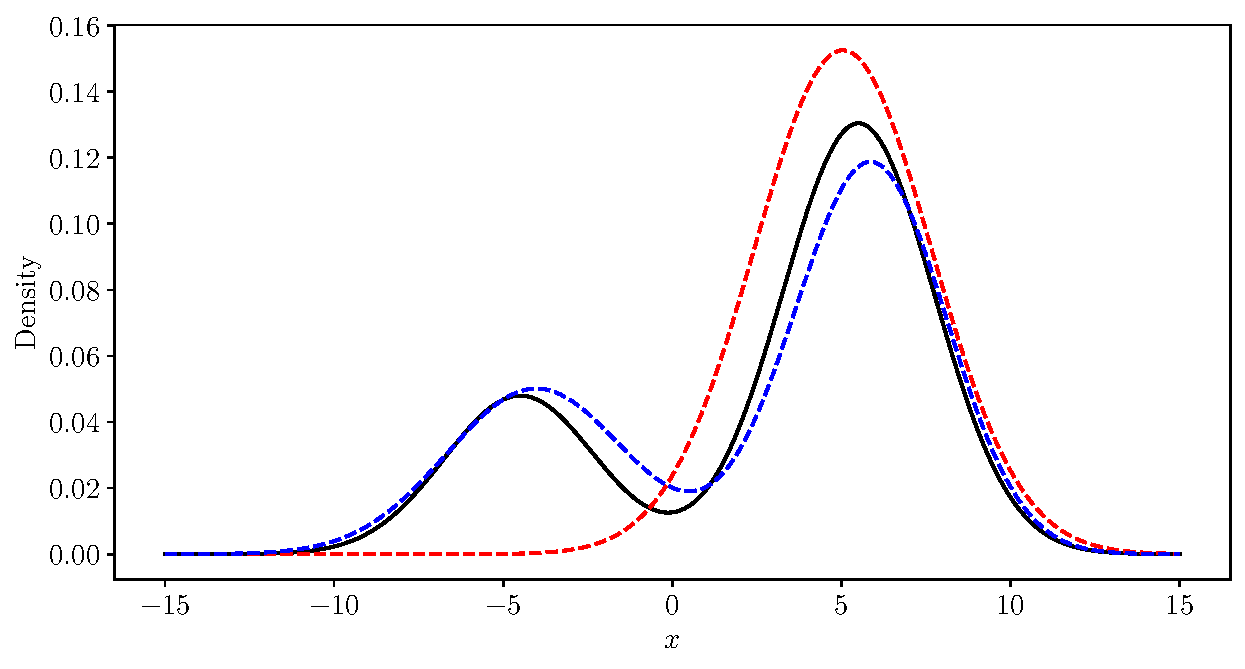
\includegraphics[width=\textwidth]{chp05_gmm/figures/bene_final_gmm}
	\caption{The mixture model algorithm implemented on the Bene\v{s} SDE \cref{eqn:bene_sde} with fixed initial condition \(x_0 = 0.5\) and over the time interval \((0,5)\).
		The probability density function of the true solution is shown in solid black and the corresponding linearisation solution in dashed red (as in \Cref{fig:bene_gauss}).
		The Gaussian mixture model density is overlaid in blue, constructed using a single split into three canonical sigma points (using \cref{eqn:uhlman_sigma}) at time \(\tau = 0.8\)).}
	\label{fig:bene_gmm}
\end{figure}

As a simple example, we apply the algorithm to the Bene\v{s} SDE \cref{eqn:bene_sde}, subject again to the initial condition \(x_0 = 1/2\) and considered at the final time of \(t = 5\).
Recall from \cref{eqn:bene_sde_pdf} and \Cref{fig:bene_gauss} that the true solution has a bimodal density, which the Gaussian distribution resulting from a single linearisation is unable to capture.
We implement the Gaussian mixture model with a single split, manually chosen to be at time \(t = 0.8\), with the resulting mixture density shown in \Cref{fig:bene_gmm}.
The algorithm is initialised with \(x^{(1)} = 1/2\), \(\Sigma^{(1)} = 0\) and \(w^{(1)}\).
After propagating the initial condition by solving \cref{eqn:gauss_de} to the splitting time \(t = 0.8\), we use the canonical sigma points (\cref{eqn:uhlman_sigma}) to replace the Gaussian density with three points \(x^{(1)}, x^{(2)}, x^{(3)}\), preserving the mean and covariance.
We then propagate these three points forward separately, in that for each one we take the deterministic trajectory \(F_{0.8}^{5}\!\left(x^{(i)}\right)\) and compute the solution to the SDE \cref{eqn:bene_sde} linearised about this trajectory.
The result is three Gaussian distributions at \(t = 5\), which we then combine as an equally weighted sum to produce a Gaussian mixture model approximating the SDE solution.
In \Cref{fig:bene_gmm}, we compare the probability density function of the resulting Gaussian mixture model to the true solution density and the Gaussian approximation from a single linearisation.
Importantly, the mixture model density includes two modes that resemble those of the true solution, which is an important feature of the solution that was not captured by the single linearisation.
Further configuration of the algorithm may result in a better fit; this was a simple and contrived example implemented to demonstrate the \emph{potential} of the mixture model algorithm in overcoming the limitations of a single Gaussian approximation.
Computing the mixture model only required the propagation of 6 values---the three means and covariance values---by solving the pair \cref{eqn:gauss_de_gmm} of differential equations three times.
We can capture the bimodality, an important feature of the solution, with only a small number of calculations.
This would be particularly advantageous in a situation where the true solution is not analytically available (as in a majority of practical scenarios) and we would have to otherwise rely on bulk simulation to observe these features.




\section{The splitting criterion}\label{sec:gmm_split_disc}
In the implementation of our algorithm on the Bene\v{s} SDE, we manually chose a single split time.
However, in general, the algorithm requires a choice of criterion for when to split a Gaussian component, for which there are several choices.
A given Gaussian component should be split when the linearised SDE is no longer a reasonable approximation for the original SDE about the deterministic trajectory corresponding to the component.
This requires an ongoing evaluation of the error in using the approximation.
Some possibilities include:
\begin{itemize}
	\item Alongside the propagation of the mixture model, one can also compute a small number of stochastic samples that solve the original SDE \cref{eqn:sde_y_gmm}.
	      These stochastic samples can be compared to the ongoing Gaussian evolutions, for instance using a probabilistic distance measure.
	      However, this would increase the computational load of the algorithm and may require many samples to accurately quantify departures from Gaussianity.
	      The Gaussian mixture model does provide an analytic probability density function that can lend itself to further inference, as opposed to solely stochastic samples that require an additional step to compute a density function.
	      There may be a trade-off between the number of samples and the desired computational efficiency.

	\item A diagnostic based purely on the deterministic model will be computationally efficient, not requiring any stochastic simulation.
	      Stochastic sensitivity (introduced by \citet{Balasuriya_2020_StochasticSensitivityComputable} and extended in \Cref{sec:theory_s2}) is a scalar value that is computed directly from the covariance matrix of the Gaussian approximation and quantifies the magnitude and direction of maximum uncertainty.
	      In highly nonlinear systems, stochastic sensitivity may provide a measure for evaluating non-Gaussianity.
	      This can be computed from each Gaussian component with minimal additional computational cost, by simply taking the operator norm of the component covariance matrix.
	      However, in regions of linearity and non-multiplicative noise, the solution to the SDE can be Gaussian, but stochastic sensitivity, being the magnitude of the noise, can increase.
	      A large value of stochastic sensitivity needs to imply non-Gaussianity in these cases.


	\item \citet{DeMarsEtAl_2013_EntropyBasedApproachUncertainty} propose an algorithm for propagating an initial uncertainty through a nonlinear time-varying mapping, by using a Gaussian mixture model and a similar splitting algorithm.
	      The principle is similar to ours; the uncertainty is propagated forward using a linearisation of the model until this is no longer a reasonable approximation.
	      A split occurs when nonlinearity in the mapping, which would result in non-Gaussianity, is detected via an entropy-based measure.
	      This measure uses the sigma point method to evaluate the mapping of a covariance matrix, which is compared to the ongoing propagation of a Gaussian component.
	      The sigma point method provides an \emph{exact} computation for the covariance matrix of a deterministic nonlinear transformation of a random variable, provided that the transformation can be evaluated exactly.
	      In our case, however, there is ongoing uncertainty from the multiplicative noise and the SDE cannot be solved exactly, so we cannot evaluate the mapping required for the sigma point method.
	      Nonetheless, this previous work may suggest a direction for further tuning the implementation of our method, including the selection of points when splitting a component.

\end{itemize}
We leave further development of this step of the algorithm for future work.




% \section{Error remains bounded}
% \note{THE PROBLEM: the mixture model at time \(t\) must be constructed from linearised SDEs all with the SAME Wiener process W_t. But then these solutions cannot possibly be independent. So the logic breaks down there.}
% \td{Check the following - important that all the linearisations used the same Wiener process. Why did I initially think this was wrong??}
% Our main result of \Cref{ch:linear_theory}, \Cref{thm:main}, establishes that the strong error in approximating the solution to a small-noise nonlinear stochastic differential equation with a linearisation is bounded by a scaling of the initial and ongoing uncertainty scales.
% In this section, we show that this result implies that if we propagate the components of a Gaussian mixture model with linearisations about the component means, as our mixture model algorithm employs, the error remains bounded in a similar fashion.

% Recall the results of \Cref{sec:theory_gauss}, the SDE linearisation theory in the special case of a Gaussian initial condition.
% Suppose that \cref{eqn:sde_no_eps} is subject to a Gaussian initial condition \(x \isGauss{\mu_0, \delta^2\Sigma_0}\), where \(\mu_0 \in \R^n\) and \(\Sigma_0 \in \R^{n\times n}\) are fixed and \(\delta > 0\) is a scaling parameter.
% We can linearise \cref{eqn:sde_no_eps} about the deterministic trajectory \(F_t^0\!\left(\mu_0\right)\) originating from the mean \(\mu_0\), as
% \begin{equation}
% 	\dif l_t\!\left(\mu_0, \delta^2\Sigma_0\right) = \begin{multlined}[t]
% 		\left[F_0^t\!\left(\mu_0\right) + \nabla u\!\left(F_0^t\!\left(\mu_0\right), t\right)\left(l_t\!\left(\mu_0, \delta^2 \Sigma_0\right) - F_0^t\!\left(\mu_0\right)\right)\right]\dif t \\
% 		+ \epsilon\sigma\!\left(F_0^t\!\left(\mu_0\right), t\right)\dif W_t, \quad l\!\left(\mu_0, \delta^2\Sigma_0\right) = x.
% 	\end{multlined}
% 	\label{eqn:scaled_sde_linear}
% \end{equation}
% We have temporarily adopted the notation \(l_t\!\left(\mu_0, \delta^2\Sigma_0\right)\) to indicate the dependence of the linearised solution on the initial mean and covariance matrix.
% The solution to \cref{eqn:scaled_sde_linear} at time \(t\) follows a Gaussian distribution with computable mean and covariance, specifically
% \[
% 	l_t\!\left(\mu, \delta^2\Sigma_0\right) \isGauss{F_0^t\!\left(\mu_0\right), \, \delta^2 \nabla F_0^t\!\left(\mu_0\right) \Sigma_0 \left[\nabla F_0^t\!\left(\mu_0\right)\right]^{\T} + \epsilon^2\Sigma_0^t\!\left(\mu_0\right)},
% \]
% where
% \[
% 	\Sigma_0^t\!\left(\mu_0\right) = \nabla F_0^t\!\left(\mu_0\right)\int_0^t{\left[\nabla F_0^\tau\!\left(\mu_0\right)\right]^{-1} \sigma\!\left(F_0^\tau\!\left(\mu_0\right), \tau\right)\sigma\!\left(F_0^\tau\!\left(\mu_0\right), \tau\right)^{\T}\left[\nabla F_0^\tau\!\left(\mu_0\right)\right]^{^{-\intercal}}\dif\tau}\left[\nabla F_0^t\!\left(\mu_0\right)\right]^{\T}.
% \]
% \Cref{thm:main} establishes that for any \(t \in [0,T]\), there exists constants \(A_1(t), A_2(t), A_3(t) \geq 0\) independent of \(\mu_0\) such that
% \begin{equation}\label{eqn:linear_error_bound}
% 	\avg{\norm{y_t - l_t\!\left(\mu_0, \delta^2 \Sigma_0\right)}} \leq A_1(t)\epsilon^2 + A_2(t)\epsilon\delta + A_3(t)\delta^2.
% \end{equation}
% Note that we have dropped the notation indicating the dependence of the constants on the coefficient bounds for notational brevity.
% Suppose at a time \(s < t\), we have a mixture model with \(M\) Gaussian components
% \[
% 	p_0\!\left(z\right) = \sum_{i=1}^{M}{\omega_i\Gauss{z;\, \mu_0^{(i)}, \delta^2\Sigma_0^{(i)}}}
% \]
% where \(\omega_1,\dotsc, \omega_M \geq 1\) are weights satisfying \(\sum_{i=1}^M{\omega_i} = 1\), \(\mu_0^{(1)}, \dots \mu_0^{(M)}\) are the component means and \(\Sigma_0^{(1)}, \dotsc, \Sigma_0^{(M)}\) are the component covariance matrices.
% Via linearisation approximations of the form \cref{eqn:scaled_sde_linear}, we construct the mixture model at time \(t > s\)
% \[
% 	p_t\!\left(z\right) = \sum_{i=1}^{M}{\omega_i\Gauss{z; \, F_s^t\!\left(\mu_0^{(i)}\right), \Pi^{(i)}}},
% \]
% where
% \[
% 	\Pi^{(i)} = \delta^2 \nabla F_0^t\!\left(\mu_0\right) \Sigma_0^{(i)} \left[\nabla F_s^t\!\left(\mu_0\right)\right]^{\T} + \epsilon^2 \Sigma_s^t\!\left(\mu_0\right),
% \]
% is the propagated covariance matrix.
% Let \(\Xi_0\) be a random variable distribution distributed according to \(p_0\), which we can write as
% \[
% 	\Xi_0 = \sum_{i=1}^{M}{I_i \xi_0^{(i)}}
% \]
% where \(\xi_0^{(i)} \isGauss{\mu_0^{(i)}, \Sigma_0^{(i)}}\) independently for each \(i\), and \(\left(I_1, \dotsc, I_M\right)\) are a set of indicator variables with
% \[
% 	P\!\left(I_i = 1,\, I_j = 0 \text{ for all } j \neq i\right) = \omega_i,
% \]
% for each \(i = 1,\hdots,M\), and zero probability otherwise.
% Similarly, let \(\Xi_t\) be a random variable distributed according the mixture model \(p_t\), which we construct from solutions to linearised SDEs of the form \cref{eqn:scaled_sde_linear}, by writing
% \[
% 	\Xi_t = \sum_{i=1}^{M}{I_i l_t\!\left(\mu_0^{(i)}, \delta^2\Sigma_0^{(i)}\right)},
% \]
% where each solution to \cref{eqn:scaled_sde_linear} is independent of the others.
% Then, for any \(i\) we have the conditional distribution
% \[
% 	\left. \Xi_t \, | \, \set{I_i = 1, \, I_j = 0 \text{ for all } j \neq i} \right. = l_{t}\left(\mu_0^{(i)}, \delta^2 \Sigma_0^{(i)}\right).
% \]
% The random variable \(\Xi_t\) represents our approximation of the state at time \(t\), after a single step of the mixture model algorithm.
% Via the law of total expectation, the error in approximating \(y_t\) with \(\Xi_t\) is
% \begin{align*}
% 	\avg{\norm{y_t - \Xi_t}} & = \sum_{i=1}^{M}{\avg{\norm{y_t - \Xi_t}\,\middle|\, I_i = 1}}P\!\left(I_i = 1,\, I_j = 0 \text{ for all } j \neq i\right) \\
% 	                         & = \sum_{i=1}^{M}{\omega_i\avg{\norm{y_t - l_{t}\left(\mu_0^{(i)}, \delta^2 \Sigma_0^{(i)}\right)}}}                        \\
% 	                         & = \sum_{i=1}^{M}{\omega_i\left(A_1(t)\epsilon^2 + A_2(t) \epsilon \delta + A_3(t)\delta^2\right)}                          \\
% 	                         & = A_1(t) \epsilon^2 + A_2(t)\epsilon\delta + A_3(t)\delta^2.
% \end{align*}
% In the mixture model algorithm described, the initialising uncertainty (being a component of the mixture model) at each step scales with \(\epsilon\), specifically \(\delta = \epsilon\).
% Thus, the error in the algorithm remains bounded with order \(\epsilon^2\).
% Note that each linearised SDE of the form \cref{eqn:scaled_sde_linear} is driven by the same Wiener process \(W_t\) as the original nonlinear SDE \cref{eqn:sde_y_gmm}.


% \td{Explain that further theory is needed}
